\section{Some Examples}

\subsection{Tables}

Notice the missing | and \verb|\hline| in the \verb|chapter2.tex| file and their effects.

% If the caption/label aren't needed, you only need the tabular environment.
\begin{table}[H]
    %\centering % Uncomment to center the table
    %\captionsetup{justification=centering} % Uncomment to center the caption
    % extra | before first l and missing | after the last l
    \begin{tabular}[b]{ || l | l  }
        \hline % "\\" adds a linebreak, "\hline" adds a horizontal line
        \textbf{Time} & \textbf{Measurement} \\\hline
        13:02 & $(20.49 \pm 0.01)\si{mm}$ \\\hline
        13:04 & $(20.47 \pm 0.01)\si{mm}$ \\%\hline
        14:32 & $(18.63 \pm 0.01)\si{mm}$ \\\hline
    \end{tabular}
    \labelcaption{table-eg}{An example table} % See appendix 1
\end{table}

\subsection{Mathematics}

% For physics units, \si{} can be used to distinguish units from variables (variables are italic).
% The "&"s control alignment. Try moving them around to adjust alignment.
\begin{align} % Use the {align*} environment instead to disable equation numbering
    % Notice how this \num{} converts its input into scientific notation
    G &\approx \num{6.674e-11}\si{N.m^{2}.kg^{-2}} \label{eq:grav-constant}\\ 
    % \num{} can also add those small spaces in large/small numbers
    \num{1000000} &= \num{1e6} = \num{1000000000000} \times \num{0.000001} \\
    % Algebra
    x &= \frac{-b \pm \sqrt{b^2 - 4ac}}{2a} \\
    % \abs, \norm, and expanding parentheses
    % _{} is for subscript, ^{} is for superscript (the {} is optional when there's 1 character)
    \norm{x}_p &= \left(\sum_i\abs{x_i}^p\right)^{\frac{1}{p}} \\
    % Matrices ("&" doesn't control alignment from within the matrix environment)
    \begin{bmatrix} 1 & 2 & 3 \\ 4 & 5 & 6 \end{bmatrix}&
        \begin{bmatrix} 7 & 8 \\ 9 & 10 \\ 11 & 12 \end{bmatrix} =
        \begin{bmatrix} 58 & 64 \\ 139 & 154 \end{bmatrix}
    % If \\ was included after the last row it'd create an extra empty line of space below
\end{align}
% Empty lines above/below an align environment will create excessive whitespace.
% A comment at the start of the line (even a "%" by itself) can prevent this.

\subsection{Graphics}

A cube with a hole through the top. Try changing the value of \texttt{cubex}.

% If the caption/label aren't needed, you only need the tikzpicture environment.
\begin{figure}[H]
    %\centering % Uncomment to center the figure
    %\captionsetup{justification=centering} % Uncomment to center the caption
    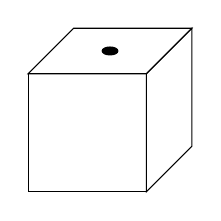
\begin{tikzpicture}
        \pgfmathsetmacro\cubex{1.5}
        \pgfmathsetmacro\cubey{1.5}
        \pgfmathsetmacro\cubez{1.5}
        \draw (0,0,0) -- ++(-\cubex,0,0) -- ++(0,-\cubey,0) -- ++(\cubex,0,0) -- cycle;
        \draw (0,0,0) -- ++(0,0,-\cubez) -- ++(0,-\cubey,0) -- ++(0,0,\cubez) -- cycle;
        \draw (0,0,0) -- ++(-\cubex,0,0) -- ++(0,0,-\cubez) -- ++(\cubex,0,0) -- cycle;
        \pgfmathsetmacro\circlex{\cubex/2}
        \pgfmathsetmacro\circlez{\cubez/2}
        \draw[fill=black] (-\circlex,0,-\circlez) ellipse (0.1 and 0.05);
    \end{tikzpicture}
    \citecaption{cube}{A cube drawn with TikZ} % See appendix 1
\end{figure}

\subsection{Lists and label references}

\begin{itemize} % itemize is for unordered lists, for ordered lists use enumerate
    \item Labels can be referenced in various ways.
    \item \verb|\ref| for figure/table/section/etc. numbers (e.g. "See figure \ref{fig:latex-logo}").
    \begin{itemize} % Sub-lists are created by nesting itemize/enumerate environments
        \item \verb|\eqref| for equation numbers (e.g. "See equation \eqref{eq:grav-constant}").
    \end{itemize}
    \item \verb|\pageref| for page numbers (e.g. "See table \ref{tab:table-eg} on page \pageref{tab:table-eg}").
\end{itemize}

\subsection{Graphs}

% If the caption/label aren't needed, you only need the tikzpicture environment.
\begin{figure}[H]
    %\centering % Uncomment to center the figure
    %\captionsetup{justification=centering} % Uncomment to center the caption
    \begin{tikzpicture}
    % Google "pgfplots gallery" to see examples of graphs and how to make them.
    % If you need negative numbers, add the "axis lines=middle" option to axis.
    \begin{axis}[
    xmin=0, xmax=1.2, ymin=0, ymax=2, % sets x-axis and y-axis limits
    xlabel={foo $a_1$ (\si{m.s^{-2}})}, % set x axis label
    ylabel={bar \\ $a_2$ (\si{m.s^{-2}})}] % set y axis label
        \addplot+[only marks,error bars/.cd,
        y dir=both,y explicit,
        x dir=both,x explicit]
        coordinates { % points
            (0.1702, 0.376) +- (0.05, 0.25)
            (0.2867, 0.552) +- (0.05, 0.25)
            (0.3886, 0.724) +- (0.05, 0.25)
            (0.4410, 0.891) +- (0.05, 0.25)
            (0.5589, 1.05)  +- (0.05, 0.25)
            (0.6659, 1.20)  +- (0.05, 0.25)
            (0.7574, 1.35)  +- (0.05, 0.25)
            (0.8580, 1.49)  +- (0.05, 0.25)
            (0.9415, 1.63)  +- (0.05, 0.25)
            (1.070,  1.77)  +- (0.05, 0.25)
        };
        % By default line domains are set to -5:5. You'll want to manually set them.
        \addplot[domain=0:2, color=black, mark=none, dotted] {2.2*x}; % dotted line
        \addplot[domain=0:2, color=black, mark=none, solid] {(1/0.541)*x}; % solid line
        \addplot[domain=0:2, color=black, mark=none, dashed] {1.5*x}; % dashed line
    \end{axis}
    \end{tikzpicture}
    \labelcaption{fancygraph}{A graph using TikZ's axis environment} % See appendix 1
\end{figure}

\subsection{Monospace text}

Some inlined paths: \lstinline{C:\Windows}, \lstinline{~/.bashrc} % \verb|| works as well

% Settings within square brackets "[]" are optional.
% The $, #, and space characters must be escaped to work properly.
\begin{cmd}[title={Some command-line commands},every listing line={\$\#>\ }]
wget http://tex.stackexchange.com
echo "is this thing working?" > test.txt
\end{cmd}
% Alternatively, import content from file
%\cmdinput{thesis-abstract.tex}[title={Paragraph 5 of the thesis abstract},listing options={firstline=20,lastline=23}]

% The starting line number is set with minted's "firstnumber".
% {python} sets the language, see https://pygments.org/docs/lexers/ for the language list.
\begin{code}{python}[title={Some Python code with syntax highlighting},minted options={firstnumber=11}]
def zip_gen(tuple_list):
    for index in range(min(len(tuple_list[0]), len(tuple_list[1]))):
        yield {tuple_list[0][index]: tuple_list[1][index]}
\end{code}
% Alternatively, import content from file
%\codeinput{thesis-abstract.tex}{latex}[title={Paragraph 3 of the thesis abstract},minted options={firstline=9,lastline=13}]

\begin{comment} % This section is hidden due to the comment environment
% {csharp} sets syntax highlighting to C#.
\begin{code}{csharp}[title={Some C\# code with syntax highlighting}]
private void StoreItemClicked(object sender, SelectionChangedEventArgs e) {
    if(Store.SelectedIndex != -1) {
        booksInCart.Add(booksInStore[Store.SelectedIndex]);
        booksInStore.RemoveAt(Store.SelectedIndex);
    }
    Refresh_ListBoxes();
}
\end{code}
\end{comment}

\subsection{Images}

A figure containing an image and a caption:
% By default, figures and tables can reorder your layout (e.g. if they go into the next page).
% Using the [H] option for figures/tables will prevent this from happening.
% To set [H] as the default for all figures, use \floatplacement{figure}{H} in the preamble.
% You could also manually reduce a figure's width or scale to fit within its page.
% If the figure caption and label aren't needed, you only need the \includegraphics command.
\begin{figure}[H]
    %\centering % Uncomment to center the image
    %\captionsetup{justification=centering} % Uncomment to center the caption
    % The image is scaled to 80% of line width (width available for text in current environment)
    
\includegraphics[width=0.8\linewidth]{LaTeX-logo.png}
    \citecaption{latex-logo}{The \LaTeX\ logo} % See appendix 1
\end{figure}
